\documentclass[a4paper, 10pt]{article}
\usepackage[margin=1in]{geometry}
\usepackage{graphicx}
\usepackage{wrapfig, tabularx, caption, hyperref}
\usepackage{cite}

\graphicspath{ {./graphs/} }

\begin{document}

\title{LZ77 report}
\author{Z0989260}
\date{\today}
\maketitle

\pagenumbering{gobble}

\newpage

\pagenumbering{arabic}

\section{Introduction}

\begin{wraptable}{r}{9.2cm}
\begin{tabularx}{9.2cm}{|X|X|X|X|}
  \hline
  filename & bytes & entropy & text\\ \hline
  
  small1.txt & 75125 & 4.648 & 26184* \\ \hline
  small2.txt & 39700 & 4.642 & 1080* \\ \hline
  small3.txt & 51185 & 4.632 & 1952* \\ \hline

  medium1.txt & 724726 & 4.575 & 1342* \\ \hline
  medium2.txt & 450783 & 4.494 & 84* \\ \hline
  medium3.txt & 234041 & 4.554 & 219* \\ \hline

  large1.txt & 1276201 & 4.599 & 2701* \\ \hline
  large2.txt & 1201891 & 4.556 & 6130* \\ \hline
  massive.txt & 5458199 & 4.602 & shkspr** \\ \hline

\end{tabularx}
\caption*{* - the 'id' of the book from www.gutenburg.org/ebooks/\textit{id}. ** - the entire works of shakespeare. Entropy is bits per byte.}
\end{wraptable}

The files I have used to demonstrate the characteristics of LZ77 can be split into four different categories, small files ($<$100kB), medium files (100kB$\geq$ x $\leq$ 800kB) and large files ($\geq$1mB). Additionally I have split 'The entire works of Shakespeare' into its own category of massive (5.46mB) due to the data yielded being significantly different to the massive category.

\begin{wrapfigure}{r}{0.5\textwidth}
  \centering
  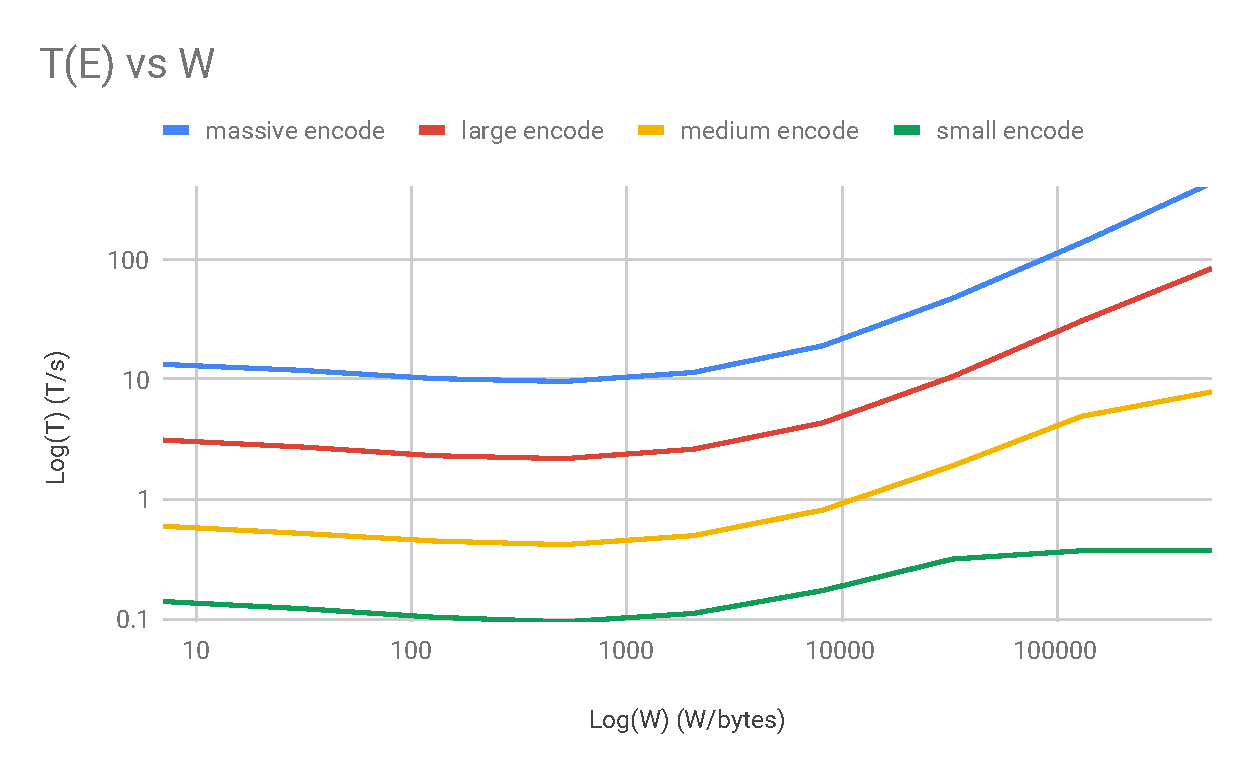
\includegraphics[width=0.5\textwidth]{TEvsW.pdf}
  \caption{Average (across each file class) of the time taken to encode each file dependant on $W$.}
\end{wrapfigure}

Additionally, I have used additional files to demonstrate the effects of LZ77 on different filetypes. These files are:
\begin{description}
\item ['.bmp'] a bitmap image of Lena commonly used in image processing,
\item ['.csv'] a '.csv' containing randomly generated data,
\item ['.flac'] a short 'free lossless audio codec' taken from a snippet of a song,
\item ['.jar'] a java archive of the hit game Minecraft.
\end{description}
The common characteristic amongst most of these files (excluding the '.jar') is that they're relatively uncompressed and high quality, hopefully leaving a lot of room for compression.

\section{Encoder running time (compression)}



The runtime of the encoder depends largely on the window size $W$ used and the size $|f|$ of the file being encoded; \textbf{Fig. 1} demonstrates the effect. Increases in file size essentially guarantee an increase in encoder running time $T(E)$, however, increasing the window size causes $T(E)$ to decrease at first (Log(W) $10-1000$) before $T(E)$ begins to rapidly climb. The logarithmic scale helps to highlight this effect. I figured this was caused by an increase in the number of \textit{self references} up to a $W$ (i.e. the encoder being able to reference itself for greater lengths as a result of being able to go further back). However, the data I set out to acquire wouldn't indicate this. To obtain this data I decided to investigate the number of instances where $l>d$ and the number of tuples written across the range $W(10-1000)$ at a greater precision (more datapoints due to a smaller increment).



The data ended up not supporting my hypothesis, the number of tuples and instances of $l>d$ read by the decoder decreased as $W$ increased (irrespective of $L$ for the most part). This lead me to believe that perhaps this isn't caused by the algorithm itself but by my implementation. In my encoder I use one loop to determine the \textit{rightmost} window match (using \textit{rfind()}) and another loop to find the longest match in the window + lookahead buffer (this one doesn't make use of \textit{rfind()}. It's possible that increasing the window size produces more rfind iterations (which are faster) up to a certain point, after which the speed begins to climb once again. The 'drop' range might depend on the entropy of the file as all the files appear to have a similar entropy (table in introduction) as they belong to a similar class (human language, short stories, etc.). Additionally it may just be the case that as $W$ grows the $T(E)$ gain resulting from writing less tuples (\textbf{Fig. 5}) completely overshadows the performance penalty of the lookahead loop.

\begin{wrapfigure}{l}{0.5\textwidth}
  \centering
  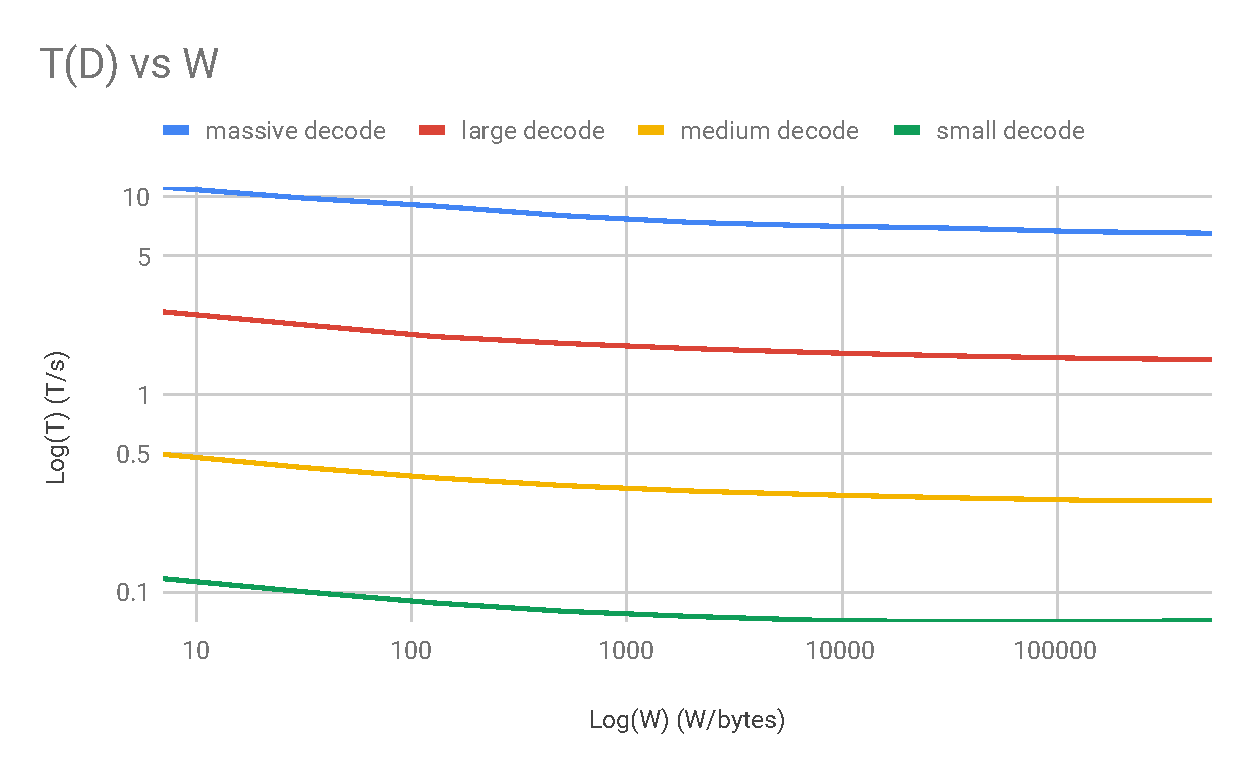
\includegraphics[width=0.5\textwidth]{TDvsW.pdf}
  \caption{Average (on each file class) of the time taken to decode depending on $W$.}
\end{wrapfigure}

This new hypothesis would be supported by the fact that the 'drop' pattern in \textbf{Fig. 1} is consistently displayed across a range of $L$ in my dataset, which would imply that there aren't that many 'lookahead matches' to be made anyway and as soon as the window increases, the \textit{rfind()} loop takes precedence. The reason for this 'power struggle' dynamic between the window and lookahead is that the 'lookahead' loop takes place directly after the 'window'/\textit{rfind()} loop and hence has its few matches stolen away.

%% talk about cases
The encoder has a worst case, best case and average case input. A best case input for the encoder is a repeating string consisting of at most one character. For example the string produced by the regex $A*$ can be encoded using two tuples if we assume $L$ to be infinite. This case can be generalised for any file type by replacing the character/string $A$ with a byte/bytes, additionally we can describe this case as the 'minimum entropy' case for our given data set. The worst case input for the encoder would consist of entirely unique string of bytes, which could also be called a maximum entropy input. However, this generalisation is limited as we might not know the distribution of the bytes / bits in our data. Additionally, we might not know if the bit / byte takes on values independent of prior input. In the example of English or any other spoken language we can attempt to model the entropy of the input based off of the probabilities of letters occuring together (and their individual probability of occuring), i.e. a 'U' is more likely to appear after a 'Q' and an 'X' is less likely to appear on its own than an 'A'. Hence if we know the distribution of the data being given, we can attempt to model an average case.

\section{Decoder running time (decompression)}

\begin{wrapfigure}{r}{0.5\textwidth}
  \centering
  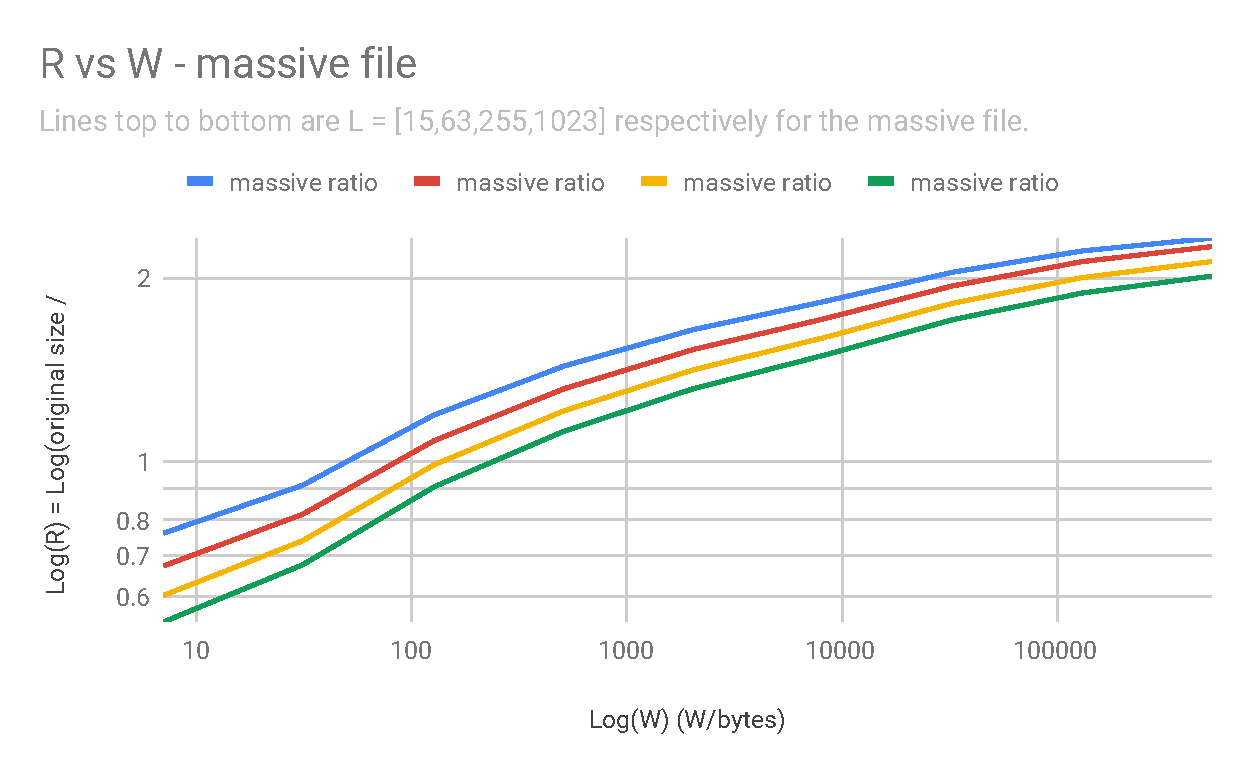
\includegraphics[width=0.5\textwidth]{RvsWmassivefile.pdf}
  \caption{Ratio of compression ($\frac{original}{encoded}$) against $W$ for the 'massive' file.}
\end{wrapfigure}

%% The runtime of the decoder is largely dependant on the parameters ($W$,$L$) used when encoding and the resulting number of tuples written. In general
In my implementation the decoder is faster than the encoder for most inputs and $T(D)$ mostly grows with $|f|$ (the size of the file) because a longer file in our data set is likelier to be more difficult to compress due to its entropy. Additionally as $W$ increases, we see a slight decrease in $T(D)$ \textbf{Fig. 2} due to the fact that a greater $W$ generally obtains a better encoding (up to a certain point) and hence the decoder has less work to do. $L$ would impact the decoder read time if it was unnecessarily increased (to the point of diminishing returns) without improving the efficiency of the encoding enough, resulting in more bits needing to be read. Otherwise, $L$ would have the potential to decrease decoding time if not for the nature of the algorithm. The most costly part of decoding is decoding from the 'so far generated' decoded string. Ideally a decoder input would consist of solely $(0,0,c)$ tuples as they are the easiest to decode, yielding the best case input (i.e. the worst case encoder input).



Similarly, the best case encoder input yields the worst case decoder input except for an empty encoder input, which would also yield a best case decoder input. A string encoded as efficiently as possible (i.e 2 tuples, representing a string $A^+$) would prove most cumbersome and take the most amount of time to decode. In summary, decoding a string encoded from a completely unique input (i.e all $(0,0,0)$ tuples) would result in a complexity of $O(n)$ where $n$ is the number of tuples to read. A string encoded as efficiently as possible would result in a complexity of $O(n^2)$. The average case would similarly depend on the statistical distribution of the data being given to the encoder.

\begin{wrapfigure}{l}{0.5\textwidth}
  \centering
  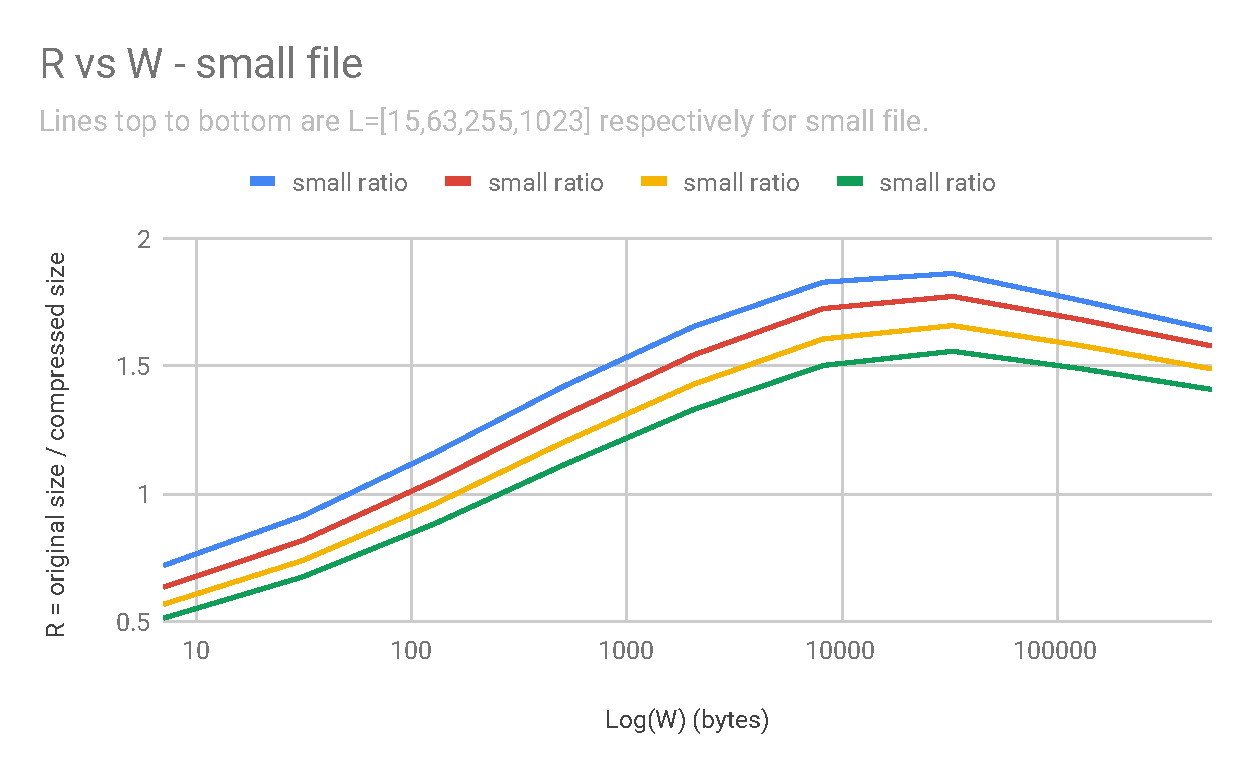
\includegraphics[width=0.5\textwidth]{RvsWsmallfile.pdf}
  \caption{Ratio of compression ($\frac{original}{encoded}$) against $W$ for the 'small' file average.}
\end{wrapfigure}

\section{Compression ratio}

\begin{wrapfigure}{r}{0.4\textwidth}
  \centering
  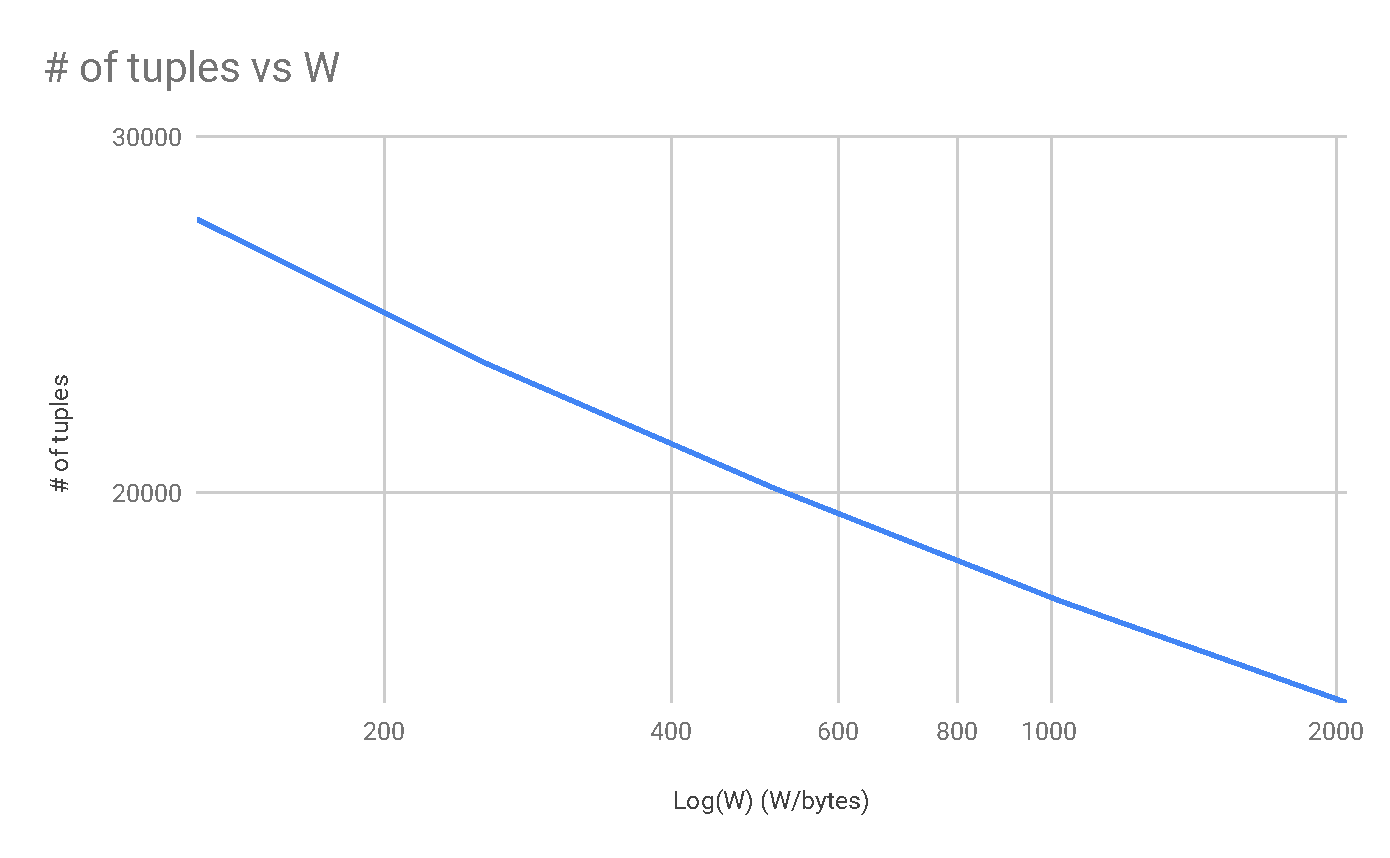
\includegraphics[width=0.4\textwidth]{TUPLESvsW.pdf}
  \caption{A graph demonstrating the relationship between the number of tuples and $W$.}
\end{wrapfigure}

\textbf{Fig. 3} and \textbf{Fig. 4} both demonstrate the effects of $W$ on compression ratio $R$. Increasing $W$ generally results in less tuples \textbf{Fig. 5} being written to the file and a better compression ratio as a result. However, there's a limit to how compactly the file can be compressed and after a certain point you recieve diminishing returns. At this point increasing $W$ yields no further compression gains and only results in a greater number of bits for $d$ in the tuple $(d,l,c)$. In fact, the number of bits stored is $\lfloor\log_2W\rfloor+1$ for any $W\geq0$. This also applies to $L$ which also suffers from diminishing returns, and at a much lower value than $W$ for most cases. Across all files I saw that the lowest $L$ was encoding best so it is likely that the large files didn't have many looping strings and consisted mostly of repeated phrases. This might explain why both algorithms utilising Huffman encoding beat my algorithm on the larger files \textit{Fig. 6}.


\section{Comparison to other algorithms}

\begin{wrapfigure}{r}{0.5\textwidth}
  \centering
  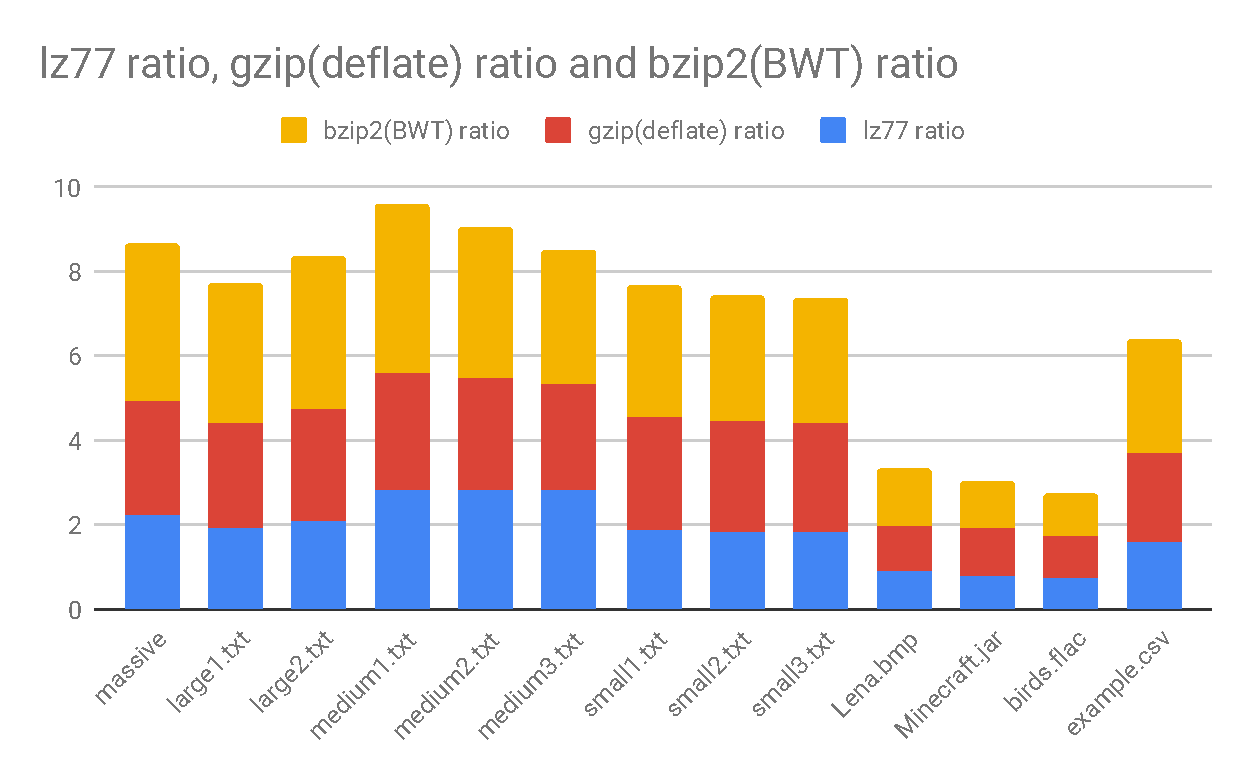
\includegraphics[width=0.5\textwidth]{comparison.pdf}
  \caption{A stacked column chart presenting the differences in compression ratio between the selected algorithms across multiple files.\\Key: Yellow - bzip, Red - gzip, Blue - lz77.}
\end{wrapfigure}

\subsection{DEFLATE (gzip)}

The Huffman part of DEFLATE can be $\theta(nlogn)$ when using a binary tree to create the dictionary\cite{huffman}, however I am unsure of the overall time complexity of DEFLATE.

\subsection{Burrows-Wheeler Transform + Huffman (bzip2)}

Im also unsure of the complexity of BWT + Huffman but in practice bzip2 appears to run slightly slower than gzip but offers a considerable boost in compression. The latter is shown in my results \textit{Fig. 6}.

\subsection{LZ77}

I can't really compare the runtime of my LZ77 encoder or decoder to the other two algorithms due to the fact that they're blazingly fast and mine is written in python. I can however compare their complexities. LZ77 is $O(n)$ (given a constant $W$ and $L$) due to the use of \textit{rfind()} which uses the $O(n+m)$ Boyer-Moore\cite{boyer} string search algorithm, where $n$ is the size of the string being searched and $m$ is the size of the string we're searching for.

In the end I found that both algorithms were able to encode most files more efficiently than my LZ77. There were some exceptions where LZ77 beat gzip, especially on the smaller files. This might mean that I could have used a greater $W$ on some of my larger files to obtain a better encoding, potentially beating gzip or making the ratios closer. I was impressed to see that my algorithm could handle all inputs apart from the '.flac' which wouldnt decode correctly but unfortunately apart from the 'example.csv' all of them encoded bigger. It's possible that all of these values had large amounts of repetition that huffman encoding was better equipped to deal with than LZ77.

\begin{thebibliography}{1}
\bibitem{huffman}
  \url{https://en.wikipedia.org/wiki/Huffman_coding}
\bibitem{boyer}
  \url{https://en.wikipedia.org/wiki/Boyer\%E2\%80\%93Moore_string-search_algorithm}
\end{thebibliography}

\end{document}
